\documentclass[11pt,a4paper]{article}

\usepackage[margin=1in]{geometry}
\usepackage{graphicx}
\usepackage{booktabs}
\usepackage{array}
\usepackage{float}
\usepackage{caption}
\usepackage{hyperref}
\usepackage{xcolor}
\usepackage{amsmath}
\usepackage{longtable}

\hypersetup{colorlinks=true,linkcolor=blue,urlcolor=blue,citecolor=blue}
\graphicspath{{report_images/}}

\title{Comparative Evaluation of Ultrasound Image Denoising Methods}
\author{Denoising Study}
\date{September 2026}

\newcommand{\method}[1]{\textbf{#1}}
\newcommand{\path}[1]{\texttt{\detokenize{#1}}}

\begin{document}
\maketitle

\begin{abstract}
This report presents a controlled comparison of ultrasound image denoising methods on 80 CETUS cardiac ultrasound slices. Synthetic multiplicative speckle noise was added to the clean images using a fixed noise level and deterministic seeds. Classical filters, a learned GRN model, and Gaussian Splatting-based models (MedGS and UltraGS) were evaluated against the original clean images using PSNR, SSIM, RMSE, ENL, CNR, and EPI. Under the fair noisy-input protocol, the Gaussian filter achieved the strongest overall denoising performance. MedGS produced only a small improvement over the noisy baseline, while the evaluated UltraGS checkpoint was preliminary because its full training stopped due to GPU memory exhaustion.
\end{abstract}

\tableofcontents
\newpage

\section{Objective}
The objective was to determine which method removes synthetic ultrasound speckle noise most effectively while preserving anatomical structure and tissue contrast. The comparison was designed around the following protocol:

\begin{enumerate}
    \item Start with an original clean ultrasound slice.
    \item Add synthetic speckle noise.
    \item Give the same noisy input to each denoising method.
    \item Compare each denoised output with the original clean slice.
    \item Aggregate the results across all 80 slices.
\end{enumerate}

The clean reference images are stored in \path{data/cetus_p01/original/}. The segmentation masks used for the ROI-based metrics are stored in \path{data/cetus_p01/seg/}.

\section{Dataset and Preprocessing}
The CETUS cardiac ultrasound sequence was extracted into 80 grayscale PNG slices:

\begin{itemize}
    \item Clean images: \path{data/cetus_p01/original/00000.png} through \path{data/cetus_p01/original/00079.png}
    \item Segmentation masks: \path{data/cetus_p01/seg/00000.png} through \path{data/cetus_p01/seg/00079.png}
    \item NeRF-style camera transforms: \path{data/cetus_p01/transforms_train.json}
\end{itemize}

For the Gaussian Splatting experiments, MedGS and UltraGS used separate copies of the noisy sequence. This kept the original clean data unchanged:

\begin{itemize}
    \item MedGS noisy dataset: \path{data/cetus_p01_medgs_noisy/original/}
    \item UltraGS noisy dataset: \path{data/cetus_p01_ultrags_noisy/images/}
\end{itemize}

Both noisy datasets contain the same 80 noisy frames.

\section{Noise Model}
Synthetic multiplicative speckle noise was generated by
\begin{equation}
    I_{\mathrm{noisy}} = I + I \cdot n,
\end{equation}
where
\begin{equation}
    n \sim \mathcal{N}(0,\sigma^2), \qquad \sigma=0.2.
\end{equation}

The noise was clipped to the valid 8-bit intensity range. For reproducibility, frame $i$ used the seed $42+i$. The implementation is in \path{utils/eval_denoising.py}, and the MedGS noisy dataset was generated by \path{scripts/prepare_medgs_noisy_dataset.py}.

\section{Methods}
\subsection{Classical Baselines}
The following 2D methods were evaluated:

\begin{itemize}
    \item Gaussian filter: OpenCV Gaussian blur with a $5\times5$ kernel and $\sigma=1.2$.
    \item Bilateral filter: OpenCV bilateral filtering with $d=7$, $\sigma_{color}=50$, and $\sigma_{space}=50$.
    \item TV-Chambolle: total variation denoising with weight $0.15$.
    \item 3D NLM: volumetric non-local means denoising with $3\times3\times3$ patches, patch distance 5, $h=0.08$, and fast mode enabled.
\end{itemize}

The classical benchmark is implemented in \path{scripts/run_denoising_benchmark.py}.

\subsection{GRN}
GRN is a UNet plus GAN denoising model. It was trained on the noisy CETUS slices and evaluated against the clean references. The representative output used in this report is \path{report_images/grn_denoised.png}. The training and evaluation script is \path{scripts/run_grn_denoising.py}.

\subsection{MedGS}
MedGS was first trained on clean images for reconstruction, producing a high reconstruction score. That result is reported separately because it is not a denoising result. MedGS was then trained again using the noisy-input dataset \path{data/cetus_p01_medgs_noisy/}. The representative fair noisy-input output used in this report is \path{report_images/medgs_noisy/00040_0.png}.

\subsection{UltraGS}
UltraGS was trained using the same noisy-input protocol and the dataset \path{data/cetus_p01_ultrags_noisy/}. An uncapped run stopped during densification because of GPU memory exhaustion. A memory-capped run then completed all 30,000 iterations by stopping densification at iteration 7,000 and using an opacity cull threshold of 0.10. The representative output used in this report is \path{report_images/ultrags_capped/00040.png}.

\section{Evaluation Metrics}
The following metrics were computed for every slice:

\begin{itemize}
    \item PSNR (dB): pixel reconstruction quality; higher is better.
    \item SSIM: structural similarity; higher is better.
    \item RMSE: pixel error; lower is better.
    \item ENL: equivalent number of looks in the target ROI; higher indicates stronger smoothing.
    \item CNR: tissue-to-background contrast; higher is better.
    \item EPI: correlation of Laplacian responses between clean and denoised images; higher indicates better edge preservation.
\end{itemize}

The metric implementations are in \path{utils/eval_denoising.py}. The segmentation mask defines the target ROI. A dilated mask ring defines the background ROI for CNR.

\section{Visual Results}
Figure~\ref{fig:classical} shows the representative slice 40 comparison for the classical methods. The clean image and noisy input are followed by the denoised results and residual maps.

\begin{figure}[H]
    \centering
    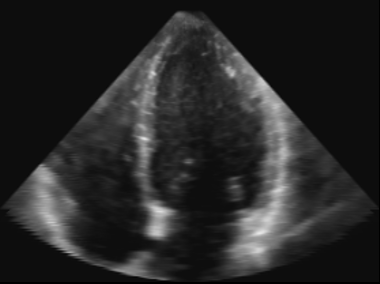
\includegraphics[width=0.48\textwidth]{clean.png}
    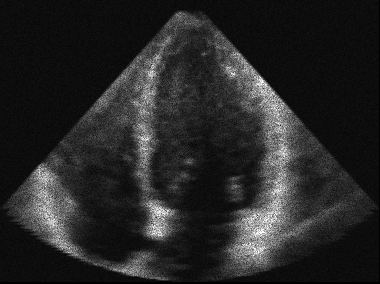
\includegraphics[width=0.48\textwidth]{noisy.png}\\
    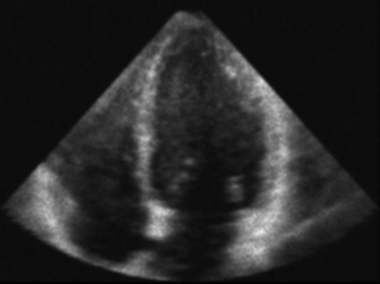
\includegraphics[width=0.48\textwidth]{gaussian_filter.png}
    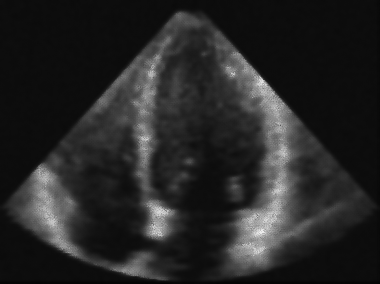
\includegraphics[width=0.48\textwidth]{bilateral_filter.png}\\
    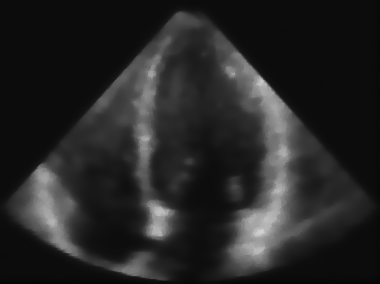
\includegraphics[width=0.48\textwidth]{tv_chambolle_filter.png}
    \caption{Representative CETUS slice 40: clean image, noisy input, Gaussian filtering, bilateral filtering, and TV-Chambolle filtering.}
    \label{fig:classical}
\end{figure}

Figure~\ref{fig:grn} shows the GRN visual comparison for slice 40.

\begin{figure}[H]
    \centering
    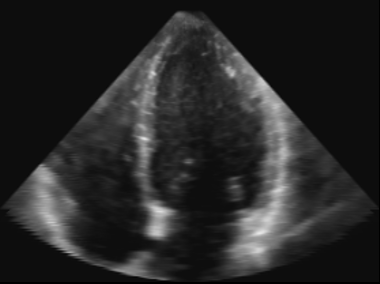
\includegraphics[width=0.48\textwidth]{clean.png}
    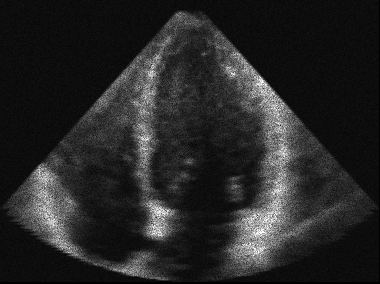
\includegraphics[width=0.48\textwidth]{noisy.png}\\
    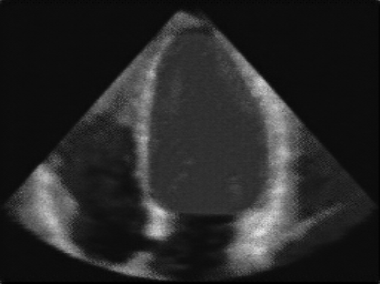
\includegraphics[width=0.48\textwidth]{grn_denoised.png}
    \caption{GRN representative result for slice 40.}
    \label{fig:grn}
\end{figure}

Figure~\ref{fig:medgs} shows the corresponding MedGS comparison using the same clean and noisy inputs.

\begin{figure}[H]
    \centering
    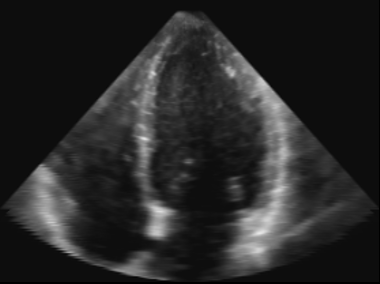
\includegraphics[width=0.48\textwidth]{clean.png}
    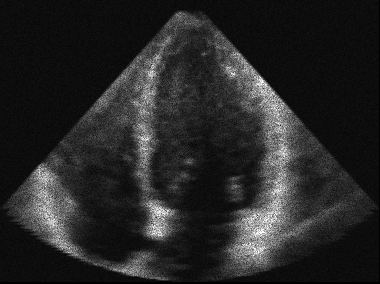
\includegraphics[width=0.48\textwidth]{noisy.png}\\
    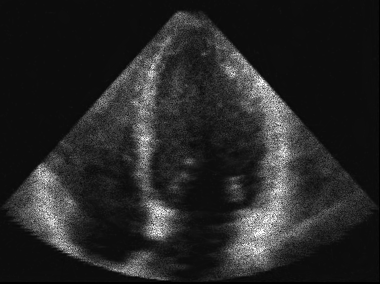
\includegraphics[width=0.48\textwidth]{medgs_noisy/00040_0.png}
    \caption{MedGS representative result for slice 40: clean image, noisy input, and denoised output.}
    \label{fig:medgs}
\end{figure}

Figure~\ref{fig:ultrags} shows the corresponding UltraGS comparison using the same clean and noisy inputs.

\begin{figure}[H]
    \centering
    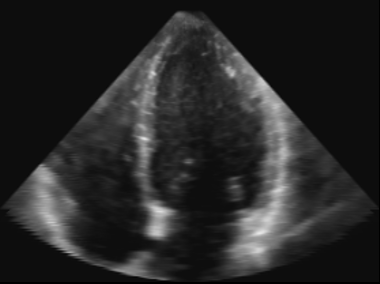
\includegraphics[width=0.48\textwidth]{clean.png}
    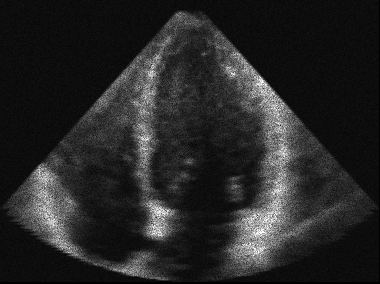
\includegraphics[width=0.48\textwidth]{noisy.png}\\
    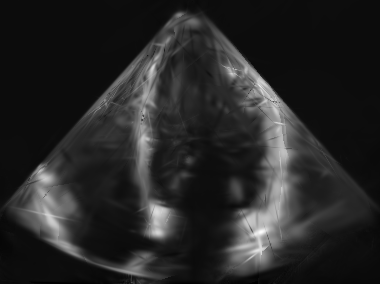
\includegraphics[width=0.48\textwidth]{ultrags_capped/00040.png}
    \caption{UltraGS representative result for slice 40: clean image, noisy input, and denoised output.}
    \label{fig:ultrags}
\end{figure}

Figure~\ref{fig:nlm} shows the corresponding 3D NLM comparison using the same clean and noisy inputs.

\begin{figure}[H]
    \centering
    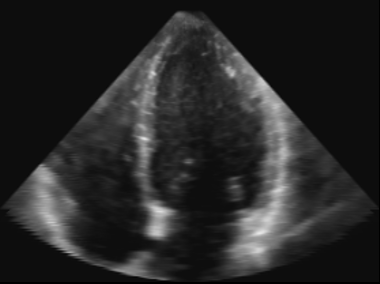
\includegraphics[width=0.48\textwidth]{clean.png}
    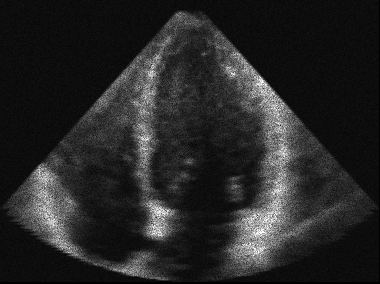
\includegraphics[width=0.48\textwidth]{noisy.png}\\
    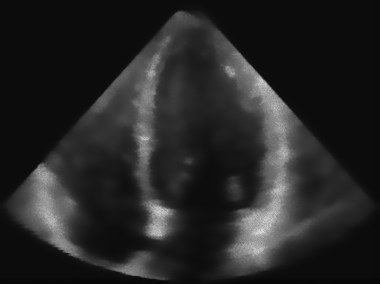
\includegraphics[width=0.48\textwidth]{3d_nlm/00040.png}
    \caption{3D NLM representative result for slice 40: clean image, noisy input, and denoised output.}
    \label{fig:nlm}
\end{figure}

The representative model-output locations are:

\begin{itemize}
    \item GRN representative output: \path{report_images/grn_denoised.png}
    \item MedGS representative output: \path{report_images/medgs_noisy/00040_0.png}
    \item UltraGS representative output: \path{report_images/ultrags_capped/00040.png}
    \item 3D NLM representative output: \path{report_images/3d_nlm/00040.png}
\end{itemize}

\section{Quantitative Results}
Table~\ref{tab:results} reports the fair denoising comparison. All rows use noisy input and comparison against the original clean image. The completed UltraGS run uses capped densification to fit the available GPU memory.

\begin{table}[H]
\centering
\caption{Fair denoising comparison across 80 CETUS slices. Values are mean $\pm$ standard deviation.}
\label{tab:results}
\small
\begin{tabular}{lrrrrrr}
\toprule
Method & PSNR $\uparrow$ & SSIM $\uparrow$ & RMSE $\downarrow$ & ENL $\uparrow$ & CNR $\uparrow$ & EPI $\uparrow$ \\
\midrule
Noisy baseline & 27.12 $\pm$ 1.12 & 0.7427 $\pm$ 0.0118 & 11.32 $\pm$ 1.49 & 3.17 $\pm$ 0.61 & 0.97 $\pm$ 0.18 & 0.126 $\pm$ 0.014 \\
Gaussian & \textbf{36.79 $\pm$ 1.25} & \textbf{0.9560 $\pm$ 0.0052} & \textbf{3.73 $\pm$ 0.53} & 4.02 $\pm$ 0.92 & 1.10 $\pm$ 0.21 & \textbf{0.497 $\pm$ 0.040} \\
Bilateral & 35.10 $\pm$ 1.49 & 0.9433 $\pm$ 0.0100 & 4.55 $\pm$ 0.77 & 4.18 $\pm$ 0.98 & 1.10 $\pm$ 0.21 & 0.191 $\pm$ 0.025 \\
TV-Chambolle & 34.38 $\pm$ 0.87 & 0.9292 $\pm$ 0.0042 & 4.89 $\pm$ 0.48 & \textbf{4.65 $\pm$ 1.15} & \textbf{1.14 $\pm$ 0.21} & 0.271 $\pm$ 0.050 \\
3D NLM & 34.11 $\pm$ 1.03 & 0.9260 $\pm$ 0.0065 & 5.06 $\pm$ 0.61 & 4.67 $\pm$ 1.10 & 1.13 $\pm$ 0.21 & 0.297 $\pm$ 0.043 \\
GRN & 27.03 $\pm$ 2.84 & 0.8654 $\pm$ 0.0130 & 12.01 $\pm$ 4.28 & \textbf{68.08 $\pm$ 12.42} & 0.97 $\pm$ 0.31 & 0.112 $\pm$ 0.013 \\
MedGS noisy input & 27.50 $\pm$ 1.18 & 0.7983 $\pm$ 0.0162 & 10.86 $\pm$ 1.50 & 3.23 $\pm$ 0.64 & 0.97 $\pm$ 0.18 & 0.138 $\pm$ 0.015 \\
UltraGS, capped 30000 iters & 25.10 $\pm$ 2.78 & 0.8180 $\pm$ 0.0408 & 14.90 $\pm$ 4.62 & 4.11 $\pm$ 1.46 & 0.95 $\pm$ 0.29 & 0.111 $\pm$ 0.062 \\
\bottomrule
\end{tabular}
\end{table}

The complete machine-readable table is in \path{output/unified_results.json}. The individual model metric files are:

\begin{itemize}
    \item Classical methods: \path{output/benchmark_results/baseline_metrics.json}
    \item GRN: \path{output/grn_results/grn_metrics.json}
    \item Clean-input MedGS reconstruction: \path{output/medgs_results/medgs_metrics.json}
    \item Fair noisy-input MedGS: \path{output/medgs_noisy_results/medgs_denoising_metrics.json}
    \item UltraGS completed capped result: \path{output/ultrags_noisy_results_capped/ultrags_denoising_metrics.json}
    \item 3D NLM: \path{output/benchmark_results/3d_nlm_metrics.json}
\end{itemize}

\section{HC-18 2D Dataset Comparison}
To test the methods on an independent fetal-head ultrasound dataset, the HC-18 training set was used as a 2D benchmark. The dataset contains 999 paired images and annotation masks. A deterministic 80/20 split was used: 799 images for GRN training and 200 held-out images for evaluation. MedGS and UltraGS were not included because they require posed image sequences for 3D Gaussian Splatting rather than independent 2D images.

The same multiplicative noise model was used with $\sigma=0.2$. Classical filters and GRN were evaluated on the held-out validation images. The benchmark implementation is in \path{scripts/run_hc18_2d_benchmark.py}, and the machine-readable results are in \path{output/hc18_2d_results/hc18_2d_metrics.json}.

\begin{figure}[H]
    \centering
    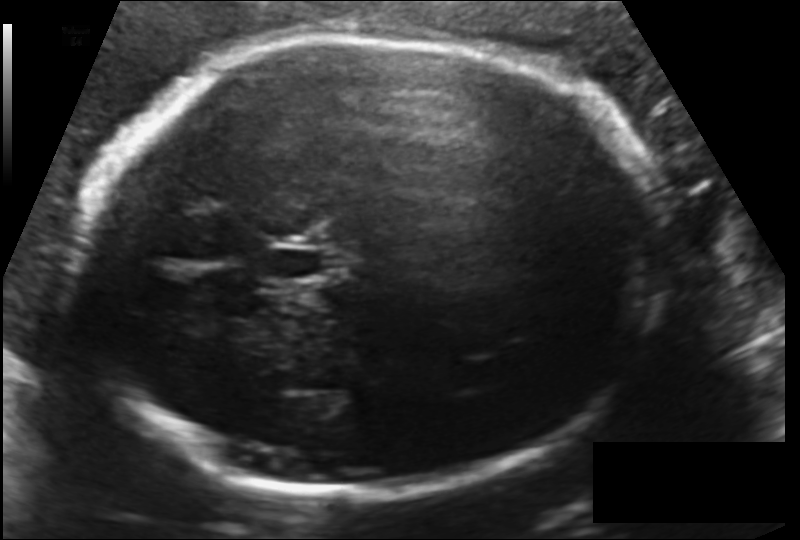
\includegraphics[width=0.48\textwidth]{hc18_2d/clean.png}
    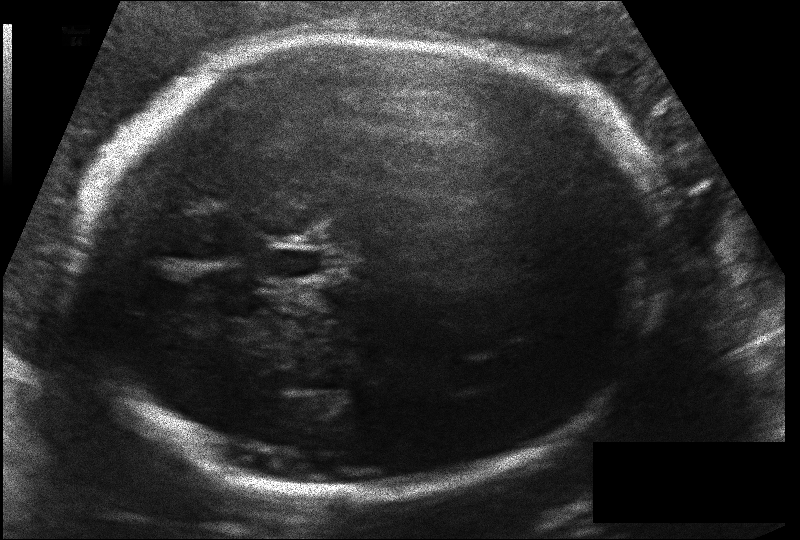
\includegraphics[width=0.48\textwidth]{hc18_2d/noisy.png}\\
    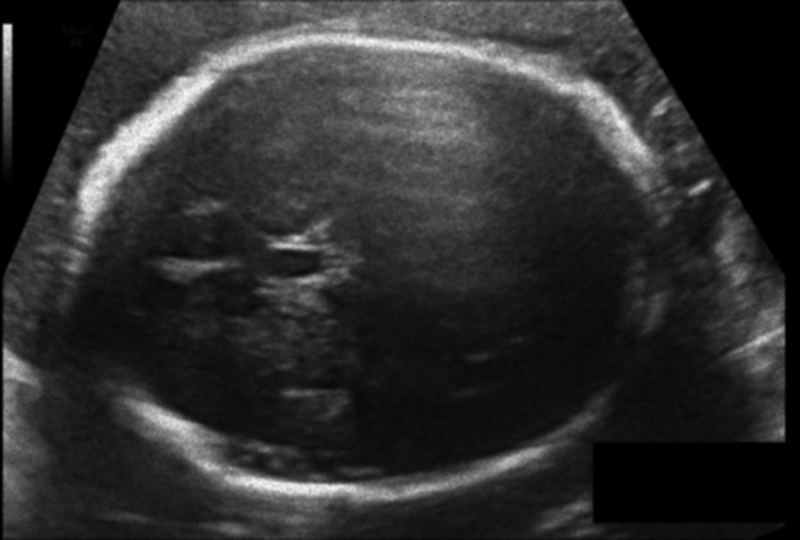
\includegraphics[width=0.48\textwidth]{hc18_2d/gaussian.png}
    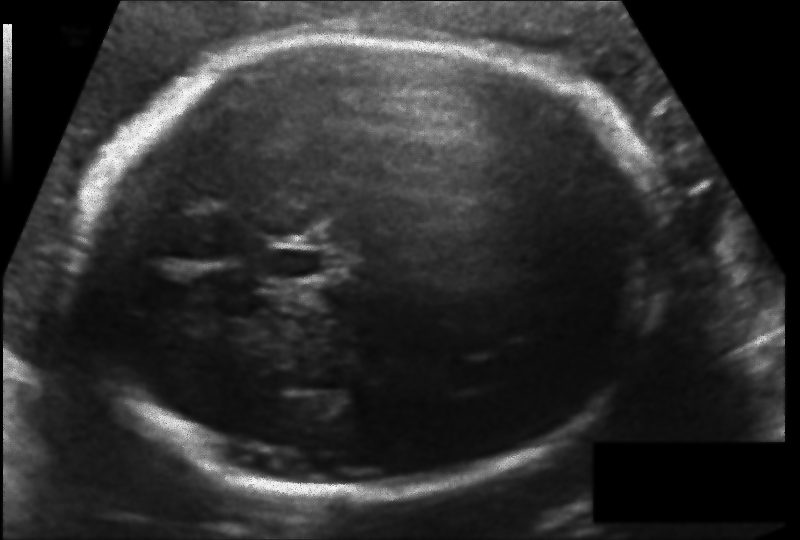
\includegraphics[width=0.48\textwidth]{hc18_2d/bilateral.png}\\
    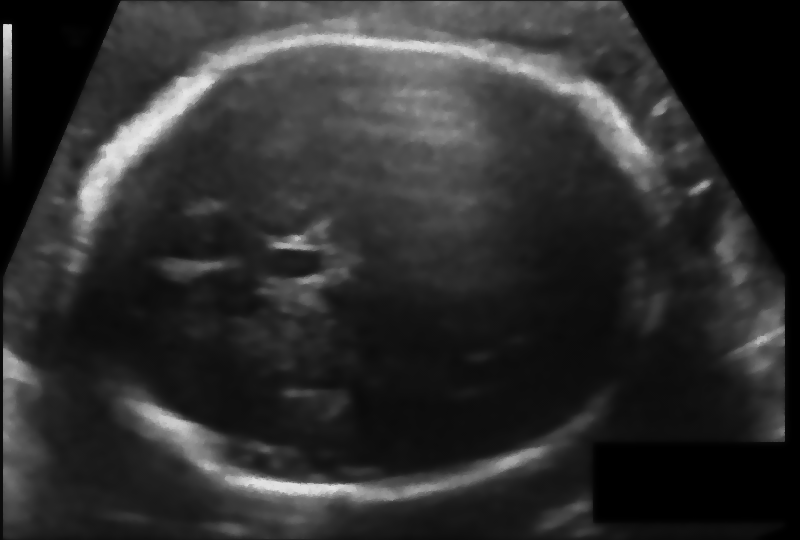
\includegraphics[width=0.48\textwidth]{hc18_2d/tvchambolle.png}
    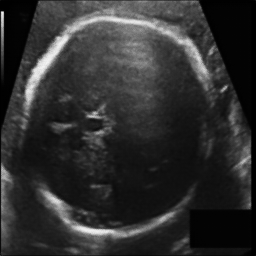
\includegraphics[width=0.48\textwidth]{hc18_2d/grn.png}
    \caption{Representative HC-18 validation image: clean image, noisy input, classical denoising outputs, and GRN output.}
    \label{fig:hc18}
\end{figure}

\begin{table}[H]
\centering
\caption{HC-18 2D denoising comparison on 200 held-out images. Values are mean $\pm$ standard deviation.}
\label{tab:hc18-results}
\small
\begin{tabular}{lrrrrrr}
\toprule
Method & PSNR $\uparrow$ & SSIM $\uparrow$ & RMSE $\downarrow$ & ENL $\uparrow$ & CNR $\uparrow$ & EPI $\uparrow$ \\
\midrule
Noisy baseline & 27.48 $\pm$ 2.20 & 0.7464 $\pm$ 0.0970 & 11.10 $\pm$ 2.58 & 2.70 $\pm$ 1.13 & 0.08 $\pm$ 0.06 & 0.076 $\pm$ 0.048 \\
Gaussian & 34.56 $\pm$ 1.68 & \textbf{0.9507 $\pm$ 0.0166} & 4.86 $\pm$ 0.93 & 3.24 $\pm$ 1.52 & 0.08 $\pm$ 0.06 & 0.338 $\pm$ 0.111 \\
Bilateral & 34.87 $\pm$ 1.62 & 0.9412 $\pm$ 0.0196 & 4.68 $\pm$ 0.87 & 3.17 $\pm$ 1.47 & 0.08 $\pm$ 0.06 & 0.104 $\pm$ 0.069 \\
TV-Chambolle & 33.92 $\pm$ 1.13 & 0.9158 $\pm$ 0.0199 & 5.18 $\pm$ 0.68 & \textbf{3.36 $\pm$ 1.60} & 0.08 $\pm$ 0.06 & 0.209 $\pm$ 0.125 \\
GRN & \textbf{36.83 $\pm$ 0.96} & 0.8691 $\pm$ 0.0639 & \textbf{3.70 $\pm$ 0.43} & 3.28 $\pm$ 1.52 & \textbf{0.31 $\pm$ 0.15} & \textbf{0.557 $\pm$ 0.088} \\
\bottomrule
\end{tabular}
\end{table}

On HC-18, GRN achieved the highest PSNR, lowest RMSE, highest CNR, and strongest EPI. The bilateral filter had slightly higher PSNR than the Gaussian filter, while the Gaussian filter achieved the highest SSIM among the denoising methods. GRN's lower SSIM despite its strong PSNR and EPI suggests that it improves pixel fidelity and edge correlation while changing some regional structural statistics. Unlike the CETUS result, GRN did not produce an unusually high ENL on HC-18; its ENL was comparable to the classical filters.

\section{Interpretation}
The Gaussian filter is the best denoising method in this experiment. It has the highest PSNR and SSIM, the lowest RMSE, and the strongest EPI among the tested methods. 3D NLM processes the full volume jointly and therefore uses inter-slice information, but its current parameters produce lower pixel fidelity than the 2D Gaussian filter. It gives high ENL and CNR, comparable to TV-Chambolle, while preserving more edges than the bilateral and TV filters.

GRN achieves an exceptionally high ENL, indicating aggressive smoothing in the selected ROI. However, its low PSNR, high RMSE, and low EPI suggest that this smoothing removes or alters useful image details. MedGS and UltraGS are Gaussian Splatting systems designed primarily for 3D scene representation, interpolation, and novel-view synthesis rather than direct 2D denoising. Under the fair noisy-input setup, neither outperformed the classical Gaussian filter. The completed capped UltraGS run improved over its earlier partial checkpoint, but remained below the noisy baseline in PSNR and RMSE.

The earlier MedGS result of 49.77 dB, 0.9962 SSIM, and 0.84 RMSE was obtained from clean-input reconstruction. It must not be used as a denoising score because the model did not receive the same noisy input as the other methods.

\section{Limitations}
\begin{itemize}
    \item The study uses 80 slices from one CETUS patient sequence.
    \item Speckle noise is synthetic rather than measured from repeated clinical acquisitions.
    \item The learned models were not pretrained specifically for this dataset.
    \item An uncapped UltraGS run exhausted GPU memory during densification; the reported UltraGS result uses a completed 30,000-iteration run with densification capped at iteration 7,000.
    \item ENL, CNR, and EPI depend on ROI selection and should be interpreted together with PSNR and SSIM.
    \item The Gaussian Splatting models may be more useful for 3D reconstruction than for this isolated 2D denoising objective.
\end{itemize}

\section{Conclusion}
For the current controlled denoising benchmark, the Gaussian filter is the strongest method by the primary fidelity metrics. 3D NLM is the fairest volume-aware classical baseline for comparison with 3D Gaussian Splatting, but it does not currently surpass Gaussian filtering numerically. GRN suppresses speckle most aggressively according to ENL, but at the cost of image fidelity. Fair noisy-input MedGS provides only a small improvement over the noisy baseline, and completed UltraGS underperforms the baseline on the primary fidelity metrics. Further work should evaluate multiple patients, real speckle noise, and task-specific 3D reconstruction quality separately from 2D denoising quality.

\end{document}
